%% capitulos/resultados.tex — Capítulo de Resultados

\chapter{Resultados}
\label{ch:resultados}

Este capítulo apresenta os resultados obtidos sobre a camada densa das redes
treinadas no MedNIST, segundo o protocolo descrito no
Capítulo~\ref{ch:metodologia}. Verifica-se, inicialmente, que a corrupção de
rótulos produziu memorização efetiva; em seguida, comparam-se as trajetórias da
LMC e das variantes de entropia amostral entre execuções com corrupção e seus
controles pareados, examinando o efeito do nível de corrupção, da arquitetura e
da ordem de achatamento dos pesos.

\section{Memorização induzida na camada densa}
\label{sec:res-desenho2}

Esta seção reporta os resultados do desenho descrito na
Seção~\ref{sec:desenho2}, no qual a perda de generalização é induzida por
corrupção de rótulos e as medidas incidem integralmente sobre os
\num{3072} pesos da camada densa. Todos os valores foram obtidos com
execuções de controle \emph{estritamente pareadas}, conforme discutido
adiante na Seção~\ref{sec:res-d2-pareamento}.

\subsection{Confirmação da memorização}
\label{sec:res-d2-memorizacao}

Antes de avaliar os indicadores, é necessário verificar que o protocolo
produziu de fato memorização, e não apenas degradação de desempenho. A
Tabela~\ref{tab:d2-memorizacao} apresenta a evidência nas oito execuções com
$\rho = 0{,}30$, isto é, \SI{25}{\percent} de rótulos efetivamente errados.

\begin{table}[H]
\centering
\caption{Evidência de memorização nas oito execuções com corrupção de rótulos
e nos oito controles pareados, em ResNet-18. Acurácias em modo de avaliação.}
\label{tab:d2-memorizacao}
\small
\begin{tabular}{lcccc}
\toprule
\textbf{Grupo} & \textbf{Treino inicial} & \textbf{Treino final} &
\textbf{Validação máxima} & \textbf{Validação final} \\
\midrule
Com corrupção ($n=8$) & \SI{74,7}{\percent} & \SI{97,5}{\percent} &
\SI{99,9}{\percent} & \SI{84,1}{\percent} \\
Controle pareado ($n=8$) & --- & \SI{100,0}{\percent} & \SI{100,0}{\percent} &
\SI{100,0}{\percent} \\
\bottomrule
\end{tabular}
\fonte{Elaborado pelo autor.}
\end{table}

O padrão é inequívoco e reprodutível nas oito execuções. A acurácia de treino
parte de aproximadamente \SI{74,7}{\percent} --- valor próximo do teto
imposto pelos rótulos corrompidos --- e sobe até \SI{97,5}{\percent}, o que
significa que a rede ajustou também a maior parte das associações
inconsistentes. Simultaneamente, a acurácia de validação, que chega a
\SI{99,9}{\percent}, regride para \SI{84,1}{\percent}. Não há explicação
visual para rótulos sorteados ao acaso; o único modo de ajustá-los é
memorizá-los. Nos controles pareados, treino e validação permanecem em
\SI{100}{\percent}, sem qualquer degradação --- o que confirma que a
memorização observada decorre da corrupção, e não do protocolo de
treinamento.

\begin{figure}[H]
    \centering
    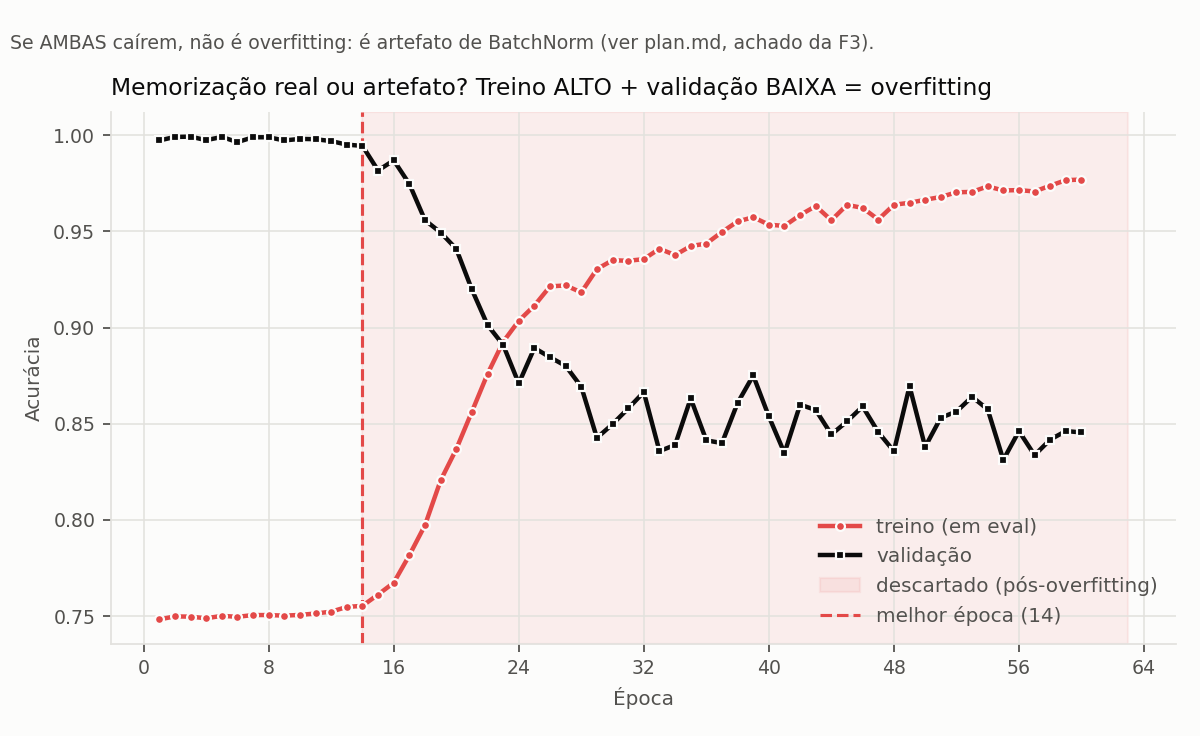
\includegraphics[width=0.9\textwidth]{figures/d2_memorizacao_resnet.png}
    \caption{Acurácias de treino, em modo de avaliação, e de validação ao longo
    das épocas em execução com \SI{25}{\percent} de rótulos efetivamente
    errados. O cruzamento das curvas caracteriza a memorização.}
    \label{fig:d2-memorizacao}
    \fonte{Elaborado pelo autor.}
\end{figure}

\subsection{Poder de discriminação dos indicadores}
\label{sec:res-d2-discriminacao}

O critério de avaliação adotado não é a amplitude absoluta de variação de cada
indicador, mas a \emph{razão} entre a amplitude observada nas execuções com
corrupção e a observada nos controles. Um indicador que varia muito nas duas
condições não informa nada sobre a memorização. A
Tabela~\ref{tab:d2-discriminacao} apresenta os resultados.

\begin{table}[H]
\centering
\caption{Amplitude de variação dos indicadores na camada densa, em ResNet-18,
com oito execuções por grupo. Valores como média $\pm$ desvio-padrão amostral;
$p$ obtido por teste de Mann-Whitney bilateral.}
\label{tab:d2-discriminacao}
\small
\begin{tabular}{lcccc}
\toprule
\textbf{Indicador} & \textbf{Com corrupção} & \textbf{Controle pareado} &
\textbf{Razão} & \textbf{$p$} \\
\midrule
LMC       & $1{,}219 \pm 0{,}055$ & $1{,}138 \pm 0{,}134$ & $1{,}07$ & $0{,}195$ \\
SampEn 1D & $0{,}205 \pm 0{,}018$ & $0{,}058 \pm 0{,}012$ & $3{,}51$ & $0{,}00016$ \\
SampEn2D  & $0{,}340 \pm 0{,}061$ & $0{,}060 \pm 0{,}014$ & $5{,}65$ & $0{,}00016$ \\
\bottomrule
\end{tabular}
\fonte{Elaborado pelo autor.}
\end{table}

O resultado é assimétrico e exige leitura cuidadosa. As duas variantes de
entropia amostral discriminam as condições, e a bidimensional discrimina
melhor. O valor $p = \num{0,00016}$ é o menor alcançável pelo teste de
Mann-Whitney com oito observações por grupo e corresponde à separação completa
entre os grupos, sem qualquer sobreposição de valores.

A complexidade LMC, em contrapartida, \textbf{não discrimina} as duas
condições. A razão de $1{,}07$ é compatível com ausência de efeito, e o teste
não rejeita a hipótese nula ($p = \num{0,195}$). Este é um resultado negativo,
e não uma limitação de potência: a amplitude média da LMC nas execuções com
corrupção ($1{,}219$) situa-se dentro de um desvio-padrão da amplitude média
dos controles ($1{,}138 \pm 0{,}134$).

A interpretação mais econômica desse achado remete à propriedade discutida na
Seção~\ref{sec:lmc}: a LMC depende apenas do histograma dos valores
dos pesos e é, portanto, invariante a qualquer permutação. Se a memorização
reorganiza os pesos da camada densa sem alterar substancialmente a
\emph{distribuição} de seus valores, a LMC é cega a ela por construção. As
variantes de entropia amostral, sensíveis à ordem, captam precisamente essa
reorganização.

\begin{figure}[H]
    \centering
    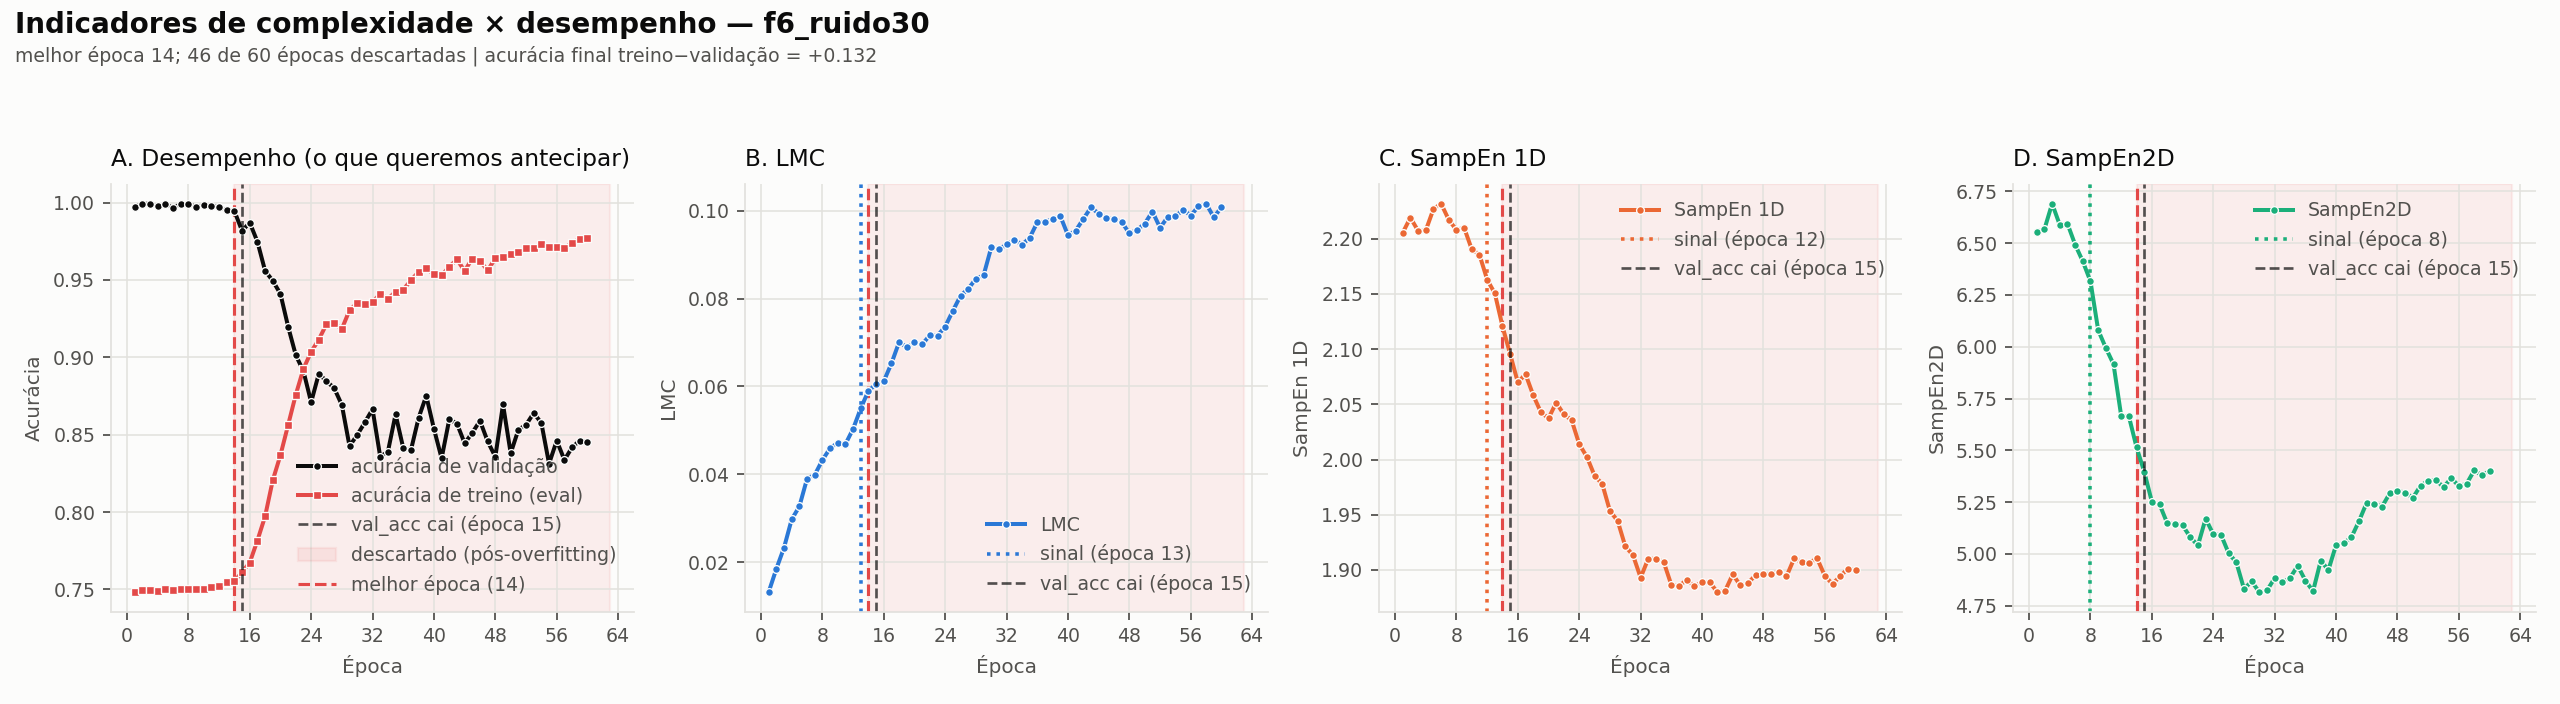
\includegraphics[width=0.95\textwidth]{figures/d2_indicadores_resnet.png}
    \caption{Trajetória dos três indicadores na camada densa e das curvas de
    validação, em execução com corrupção de rótulos. A região sombreada
    corresponde às épocas posteriores ao início do sobreajuste, excluídas das
    conclusões.}
    \label{fig:d2-indicadores}
    \fonte{Elaborado pelo autor.}
\end{figure}

\subsection{Antecedência em relação à degradação da validação}
\label{sec:res-d2-antecedencia}

A antecedência é a diferença, em épocas, entre a inflexão do indicador e a
âncora definida sobre a acurácia de validação. A
Tabela~\ref{tab:d2-antecedencia} reporta os valores.

\begin{table}[H]
\centering
\caption{Antecedência dos indicadores em relação à queda sustentada da acurácia
de validação, em épocas, nas oito execuções com corrupção em ResNet-18.}
\label{tab:d2-antecedencia}
\small
\begin{tabular}{lccc}
\toprule
\textbf{Indicador} & \textbf{Média $\pm$ desvio} & \textbf{IC \SI{95}{\percent}} &
\textbf{Discrimina?} \\
\midrule
SampEn2D  & $7{,}50 \pm 0{,}93$ & $[6{,}73;\ 8{,}27]$ & Sim \\
SampEn 1D & $3{,}62 \pm 1{,}06$ & $[2{,}74;\ 4{,}51]$ & Sim \\
LMC       & $3{,}00 \pm 1{,}85$ & $[1{,}45;\ 4{,}55]$ & Não \\
\bottomrule
\end{tabular}
\fonte{Elaborado pelo autor.}
\end{table}

A antecedência da LMC não constitui resultado positivo e não deve ser
interpretada como tal. Como a Tabela~\ref{tab:d2-discriminacao} estabelece que
o indicador não distingue as duas condições, a época de sua inflexão não
sinaliza coisa alguma: uma inflexão que ocorre igualmente nos controles não é
aviso. A antecedência só é informativa para indicadores que previamente
demonstraram discriminação.

A separação temporal da SampEn2D é quase completa. Nas oito execuções com
corrupção, o indicador inflete nas épocas $\{7,7,7,7,7,7,8,9\}$. Nos controles
pareados, seis dos oito inflectem, e o fazem nas épocas
$\{9,23,37,42,50,55\}$; os dois restantes não inflectem dentro do horizonte de
\num{60} épocas. Registre-se a honestidade do limite: há \emph{um} controle que
inflete na época \num{9}, coincidindo com o valor máximo observado no grupo com
corrupção. A separação é portanto quase perfeita, mas não perfeita, e a
afirmação correta é de sobreposição mínima --- em uma de dezesseis execuções.

\subsection{Efeito do nível de corrupção}
\label{sec:res-d2-niveis}

Variou-se a fração sorteada em $\rho \in \{0{,}15;\ 0{,}30;\ 0{,}50\}$, com três
sementes por nível. O resultado não era o esperado e é, talvez, o mais
interessante desta seção.

\begin{table}[H]
\centering
\caption{Época do alerta emitido pelo monitor e época da âncora, por nível de
corrupção, com três sementes por nível.}
\label{tab:d2-niveis}
\small
\begin{tabular}{lcccc}
\toprule
\textbf{$\rho$ sorteado} & \textbf{Errados de fato} & \textbf{Época do alerta} &
\textbf{Época da âncora} & \textbf{Antecedência} \\
\midrule
\SI{15}{\percent} & \SI{12,5}{\percent} & $10{,}0$ & $17{,}7$ & $7{,}7$ \\
\SI{30}{\percent} & \SI{25,0}{\percent} & $9{,}3$  & $14{,}7$ & $5{,}3$ \\
\SI{50}{\percent} & \SI{41,7}{\percent} & $10{,}0$ & $13{,}0$ & $3{,}0$ \\
\midrule
\multicolumn{2}{l}{ANOVA de uma via} & $F = 1{,}00$ & $F = 30{,}2$ & \\
\multicolumn{2}{l}{} & $p = 0{,}42$ & $p = 0{,}0007$ & \\
\bottomrule
\end{tabular}
\fonte{Elaborado pelo autor.}
\end{table}

A época em que o monitor emite o alerta é praticamente invariante ao nível de
corrupção: médias de $10{,}0$, $9{,}3$ e $10{,}0$ épocas, sem diferença
estatisticamente detectável ($F = \num{1,00}$; $p = \num{0,42}$). O que se move
é a âncora, isto é, o momento em que a degradação se torna visível na
validação, que chega progressivamente mais cedo quanto maior a corrupção
($F = \num{30,2}$; $p = \num{0,0007}$).

A consequência prática é que a antecedência encolhe à medida que a corrupção
aumenta, de aproximadamente $7{,}7$ épocas a \SI{15}{\percent} para $3{,}0$
épocas a \SI{50}{\percent}. Propõe-se a seguinte leitura: o indicador marca o
\emph{início} da memorização, cujo momento depende pouco da quantidade de
rótulos errados, enquanto a validação mede o \emph{sintoma}, que se manifesta
tanto mais cedo quanto maior a corrupção. Trata-se de interpretação
plausível e compatível com os dados, ainda não demonstrada de forma
independente.

\begin{figure}[H]
    \centering
    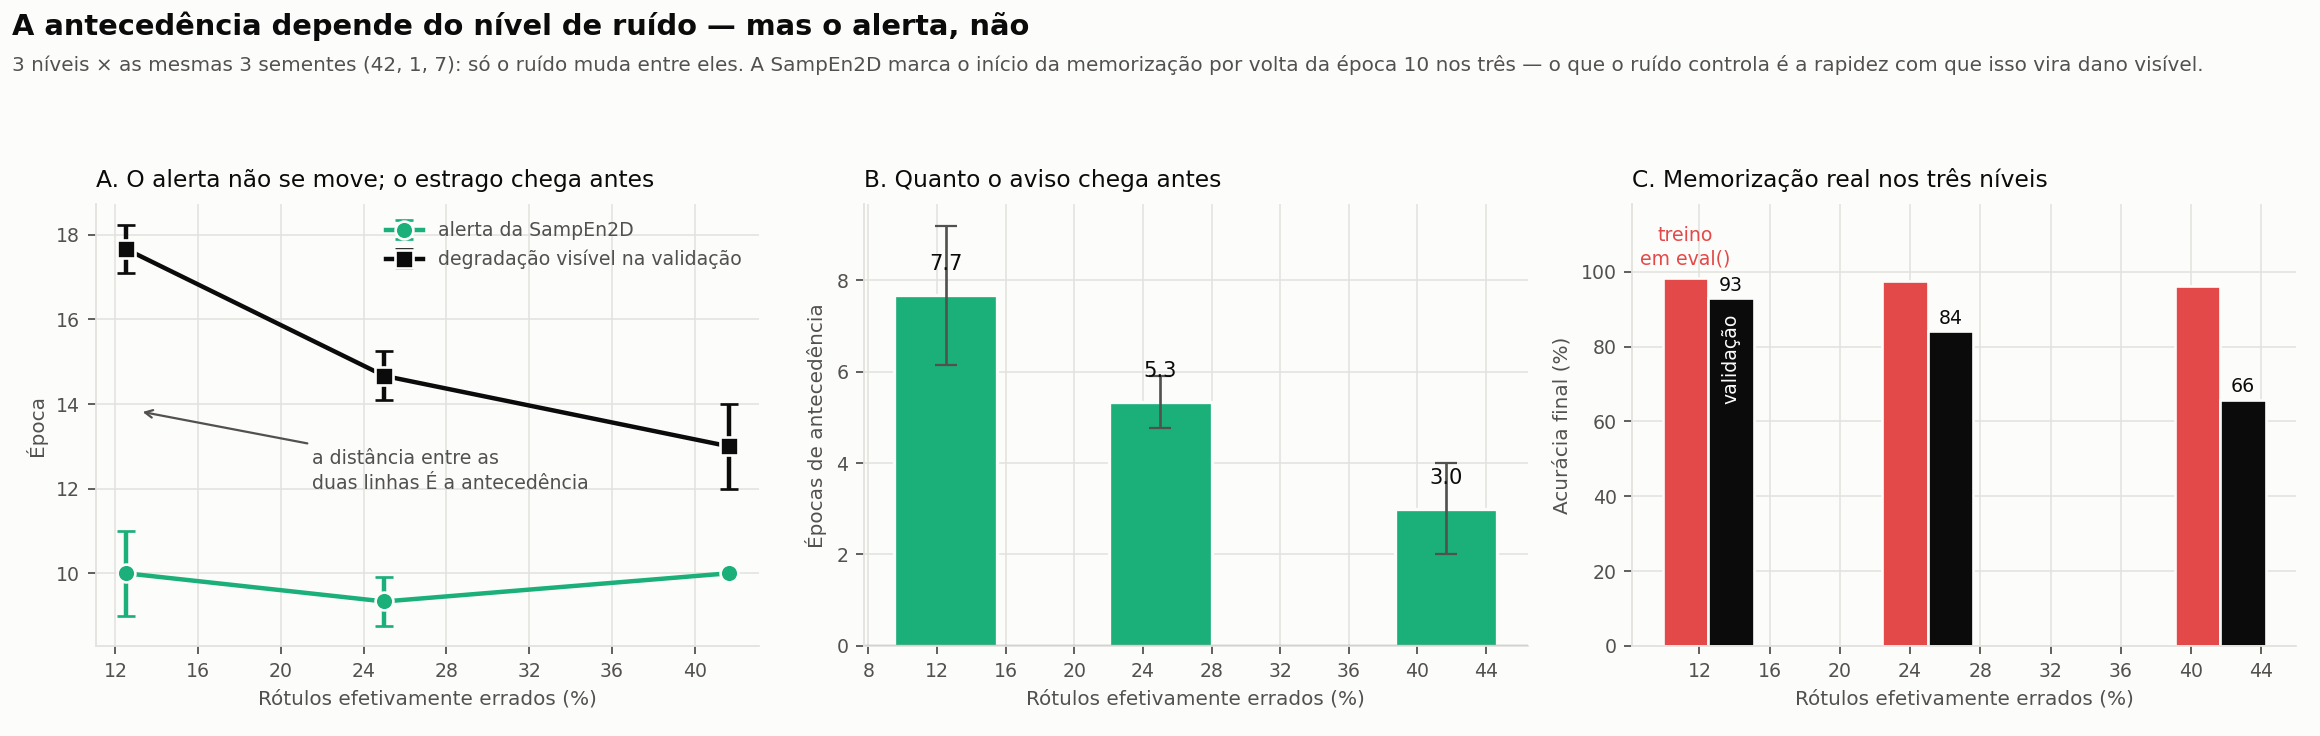
\includegraphics[width=0.9\textwidth]{figures/d2_niveis_ruido.png}
    \caption{Época do alerta e época da âncora em função do nível de corrupção
    de rótulos. A época do alerta é estável; a da âncora antecipa-se com o
    aumento da corrupção.}
    \label{fig:d2-niveis}
    \fonte{Elaborado pelo autor.}
\end{figure}

\subsection{Generalização para outra arquitetura}
\label{sec:res-d2-arquitetura}

O experimento foi repetido com a DenseNet-121, com oito execuções com
corrupção e cinco controles pareados. Os resultados constam da
Tabela~\ref{tab:d2-densenet}.

\begin{table}[H]
\centering
\caption{Resultados na DenseNet-121, com oito execuções com corrupção e cinco
controles pareados.}
\label{tab:d2-densenet}
\small
\begin{tabular}{lccc}
\toprule
\textbf{Indicador} & \textbf{Razão de amplitude} & \textbf{$p$} &
\textbf{Antecedência (épocas)} \\
\midrule
LMC       & $1{,}06$ & $0{,}435$   & --- \\
SampEn 1D & $1{,}77$ & $0{,}00155$ & $22{,}50 \pm 2{,}33$ \\
SampEn2D  & $4{,}35$ & $0{,}00155$ & $21{,}12 \pm 2{,}36$ \\
\bottomrule
\end{tabular}
\fonte{Elaborado pelo autor.}
\end{table}

O achado central replica-se na segunda arquitetura. A SampEn2D discrimina com
razão de $4{,}35$ vezes ($p = \num{0,00155}$) e a antecedência é
consideravelmente maior, de $21{,}1 \pm 2{,}4$ épocas, com intervalo de
confiança de \SI{95}{\percent} entre $19{,}2$ e $23{,}1$. A LMC, de novo, não
discrimina ($p = \num{0,435}$), o que reforça a consistência desse resultado
negativo entre arquiteturas.

Duas ressalvas, porém, devem ser explicitadas.

A primeira é que a razão de amplitude é menor do que na ResNet-18
($4{,}35$ contra $5{,}65$), e a SampEn 1D, que discriminava na ResNet, passa a
ter poder marginal ($1{,}77$). O contraste, portanto, replica-se em direção,
mas não em magnitude.

A segunda é mais relevante e não deve ser omitida: \textbf{na DenseNet-121 a
época do sinal não separa os grupos}. As execuções com corrupção inflectem nas
épocas $\{8,9,9,9,9,11,11,12\}$, enquanto os controles pareados inflectem em
$\{7,8,10,16,25\}$ --- três deles, portanto, tão cedo ou mais cedo que as
execuções com corrupção. Na ResNet-18 a separação temporal é quase perfeita; na
DenseNet-121, não existe. O que discrimina nessa arquitetura é a
\emph{amplitude} da variação, não o \emph{momento} em que ela começa. A
consequência prática é direta: um monitor que emita alerta pelo simples cruzamento
de um limiar temporal produziria falsos positivos na DenseNet-121, e o critério
precisa incorporar a magnitude.

\begin{figure}[H]
    \centering
    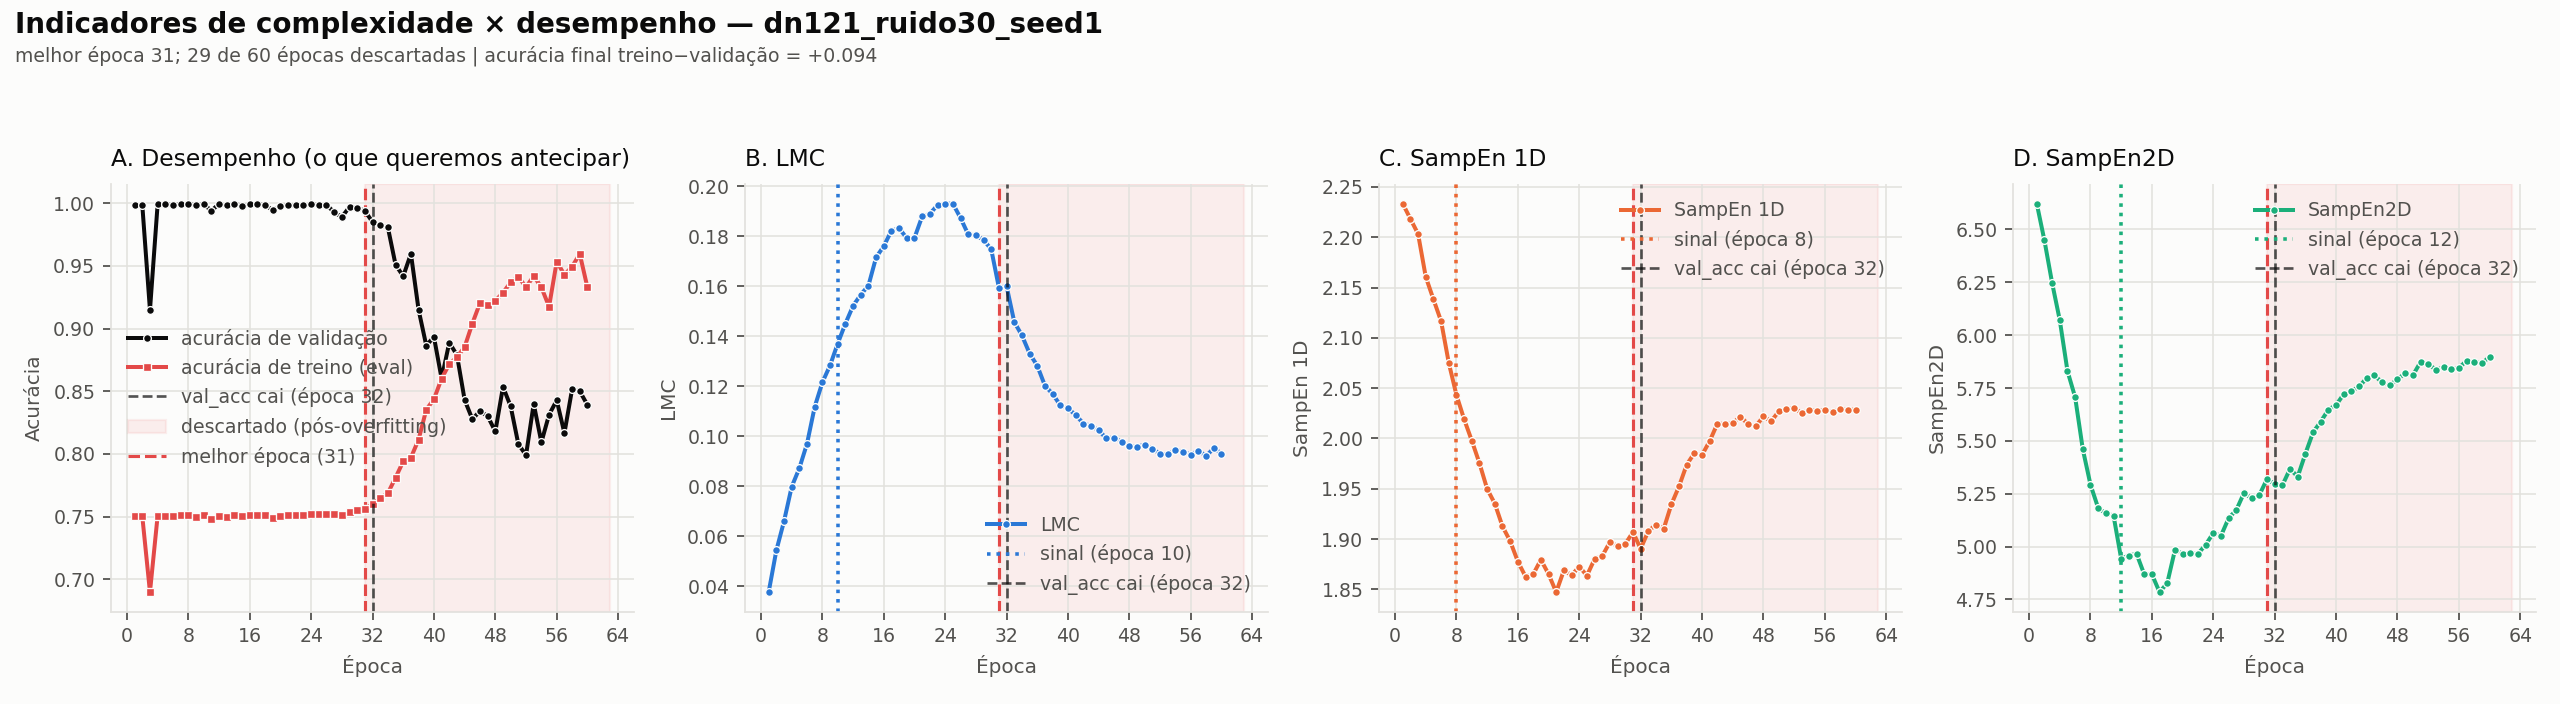
\includegraphics[width=0.95\textwidth]{figures/d2_indicadores_dn121.png}
    \caption{Trajetória dos indicadores na camada densa da DenseNet-121, em
    execução com corrupção de rótulos.}
    \label{fig:d2-dn121}
    \fonte{Elaborado pelo autor.}
\end{figure}

\subsection{Ablação da ordem de achatamento}
\label{sec:res-d2-ablacao}

A Seção~\ref{sec:camada-densa} fixou a ordem por neurônio como convenção
padrão, por coerência com a decisão D2, e previu o reporte da comparação com a
ordem por entrada. A Tabela~\ref{tab:d2-ablacao} apresenta o resultado, obtido
sobre cinco execuções com corrupção e cinco controles.

\begin{table}[H]
\centering
\caption{Comparação das duas ordens de achatamento na SampEn 1D da camada densa.}
\label{tab:d2-ablacao}
\small
\begin{tabular}{lcc}
\toprule
\textbf{Ordem} & \textbf{Razão de amplitude} & \textbf{Antecedência (épocas)} \\
\midrule
Por neurônio (padrão adotado) & $3{,}52$ & $3{,}6$ \\
Por entrada                   & $7{,}73$ & $7{,}4$ \\
\bottomrule
\end{tabular}
\fonte{Elaborado pelo autor.}
\end{table}

O resultado contraria a convenção adotada, e isso precisa ser dito sem
atenuação: a leitura \emph{por entrada} é superior nos dois critérios,
discriminando mais que o dobro ($7{,}73$ contra $3{,}52$) e avisando com o dobro
da antecedência ($7{,}4$ contra $3{,}6$ épocas).

Há uma explicação plausível. Percorrer a matriz por entrada agrupa, para cada
característica, os pesos que ela envia a \emph{todas} as classes --- e é
exatamente aí que a memorização se manifesta, quando uma característica passa a
apontar de forma desproporcional para uma classe específica. Percorrendo por
neurônio, esse contraste dilui-se ao longo das \num{512} posições do campo
receptivo.

Registre-se que o efeito prático dessa escolha é limitado, pois o indicador de
melhor desempenho neste trabalho é a SampEn2D, que não achata a matriz e
preserva as duas direções simultaneamente. A discussão de ordem afeta apenas a
variante unidimensional. Ainda assim, a evidência recomenda reconsiderar a
convenção adotada.

\subsection{Sobre o pareamento dos controles}
\label{sec:res-d2-pareamento}

Um aspecto metodológico merece registro explícito, por afetar a validade de
todos os números desta seção.

Em uma versão anterior deste conjunto de experimentos, as execuções de controle
não eram estritamente pareadas: além de não terem rótulos corrompidos, elas
empregavam aumento de dados, decaimento de pesos de $10^{-4}$ e horizonte de
\num{40} épocas, contra ausência de aumento, decaimento nulo e \num{60} épocas
nas execuções com corrupção. Como aumento de dados e decaimento de pesos são,
ambos, formas de regularização que reduzem sobreajuste por conta própria, o
contraste medido era atribuível a mais de uma causa, e não exclusivamente à
memorização.

Todo o conjunto de controles foi então refeito com pareamento estrito, e os
números reportados nesta seção são os dessa segunda versão. A comparação entre
as duas consta da Tabela~\ref{tab:d2-pareamento}.

\begin{table}[H]
\centering
\caption{Efeito da correção do pareamento sobre as razões de amplitude da
SampEn2D.}
\label{tab:d2-pareamento}
\small
\begin{tabular}{lccc}
\toprule
\textbf{Arquitetura} & \textbf{Controles não pareados} &
\textbf{Controles pareados} & \textbf{$p$ final} \\
\midrule
ResNet-18    & $5{,}71$ ($n=8$) & $5{,}65$ ($n=8$) & $0{,}00016$ \\
DenseNet-121 & $2{,}80$ ($n=3$) & $4{,}35$ ($n=8$) & $0{,}00155$ \\
\bottomrule
\end{tabular}
\fonte{Elaborado pelo autor.}
\end{table}

Na ResNet-18 a razão praticamente não se alterou, passando de $5{,}71$ para
$5{,}65$. Esse é um resultado importante em si: como a correção removeu a
regularização dos controles e o contraste permaneceu, conclui-se que o efeito
medido decorre da memorização, e não das diferenças de regularização. Na
DenseNet-121 a razão \emph{aumentou}, de $2{,}80$ para $4{,}35$, e passou a ser
estatisticamente significativa --- o que indica que a aparente fraqueza dessa
arquitetura, registrada em análise preliminar, era em boa parte artefato do
pareamento inadequado, agravado pelo número reduzido de execuções.
